\documentclass{beamer}
\usetheme{Singapore}
\usepackage{changepage}

%\usepackage{pstricks,pst-node,pst-tree}
\usepackage{amssymb,latexsym,dirtree}
\usepackage{tikz}
\usepackage{graphicx}
\usepackage{fancyvrb}
\usepackage{hyperref}
\usepackage{fancybox}
\usepackage[listings]{tcolorbox}

\definecolor{codegreen}{rgb}{0,0.6,0}
\definecolor{codegray}{rgb}{0.5,0.5,0.5}
\definecolor{codepurple}{rgb}{0.58,0,0.82}
\definecolor{backcolour}{rgb}{0.95,0.95,0.92}

\lstdefinestyle{mystyle}{
    language=Python,
    backgroundcolor=\color{backcolour},   
    commentstyle=\color{codegreen},
    keywordstyle=\color{magenta},
    numberstyle=\tiny\color{codegray},
    stringstyle=\color{codepurple},
    basicstyle=\ttfamily\normalsize,
    breakatwhitespace=false,         
    breaklines=true,                 
    captionpos=b,                    
    keepspaces=true,                 
    numbers=left,                    
    numbersep=5pt,                  
    showspaces=false,                
    showstringspaces=false,
    showtabs=false,                  
    tabsize=2,
    escapechar=|,
    frame=single
}

\lstset{style=mystyle}

\newcommand{\lst}[1]{\lstinline{#1}}


\newcommand{\bi}{\begin{itemize}}
\newcommand{\li}{\item}
\newcommand{\ei}{\end{itemize}}
\newcommand{\Show}[1]{
\begin{center}
\shadowbox{\begin{minipage}{0.8\textwidth}
          #1
          \end{minipage}}
\end{center}
}
\newcommand{\arrow}{\ensuremath{\rightarrow}}

\newcommand{\uparr}{\ensuremath{\uparrow}}


\newcommand{\fig}[2]{\centerline{\includegraphics[width=#1\textwidth]{#2}}}

\newcommand{\bfr}[1]{\begin{frame}[fragile]\frametitle{{ #1 }}}
\newcommand{\efr}{\end{frame}}

\newcommand{\cola}{\begin{columns}\begin{column}{0.5\textwidth}}
\newcommand{\colb}{\end{column}\begin{column}{0.5\textwidth}}
\newcommand{\colc}{\end{column}\end{columns}}


\title{\url{https://intro2r.com/} Chapter 1}
\author{CSCI 297b, Spring 2023}

\begin{document}

\begin{frame}
\maketitle
\end{frame}

\bfr{Advantages of R}
\begin{itemize}
\item
R is open source and freely available.
\item
R is available for Windows, Mac and Linux operating systems.
\item
R has an extensive and coherent set of tools for statistical analysis.
\item
R has an extensive and highly flexible graphical facility capable of producing publication quality figures.
\item
R has an expanding set of freely available ‘packages’ to extend R’s capabilities.
\item
R has an extensive support network with numerous online and freely available documents.
\end{itemize}
\end{frame}

\bfr{RStudio panels}

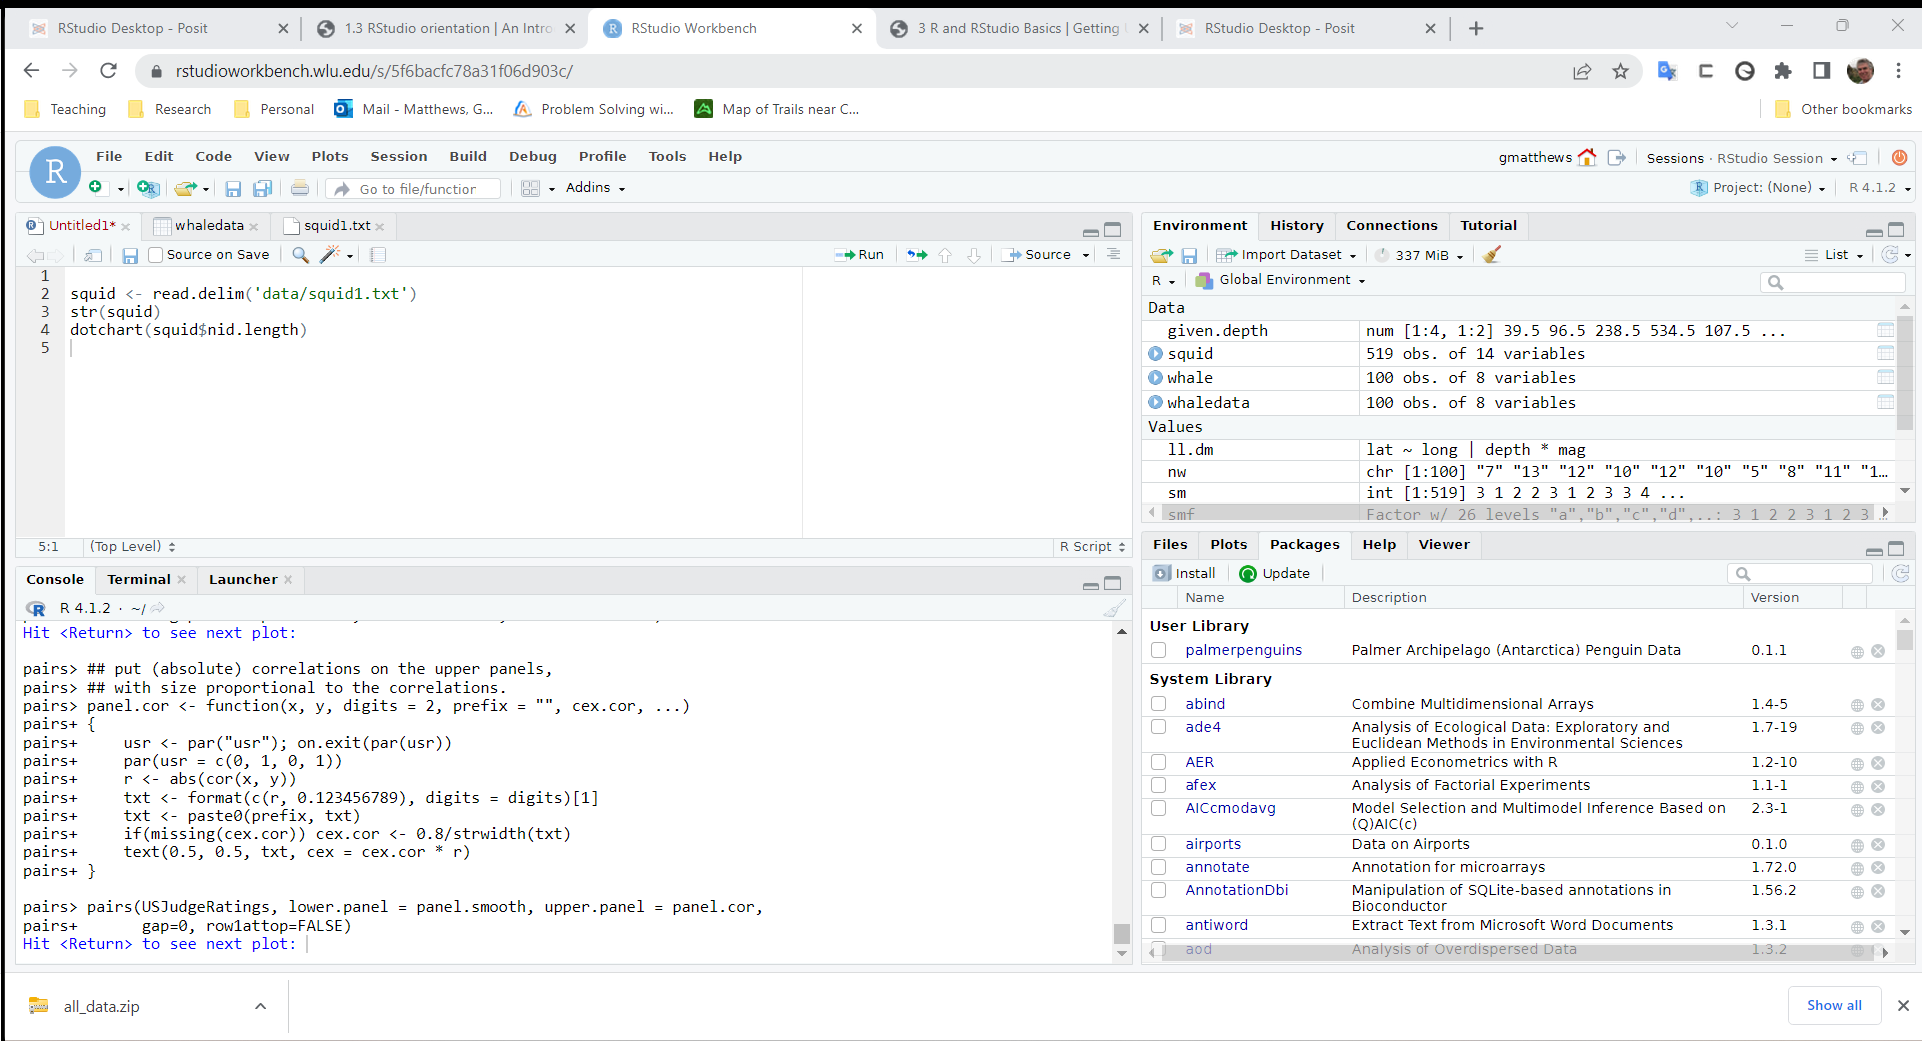
\includegraphics[width=\textwidth]{rstudioscreen}

\end{frame}

\bfr{RStudio panels left side}
\begin{itemize}
\item Source window
\begin{itemize}
\item Enter and edit commands for the R interpreter.
\item Not sourced into the R interpreter until you hit \fbox{\sf Source} button.
\item Can be sourced with control+enter (windows) or command+enter (mac)
\end{itemize}
\item {Console/Terminal/Launcher window}
\begin{itemize}
\item Type commands directly into the R interpreter.
\item Use as a calculator
\end{itemize}
\end{itemize}

\end{frame}
\bfr{RStudio panels right side}
\begin{itemize}
\item Environment/History/Connections/Tutorial window
\begin{itemize}
\item Environment tells you what names you have defined.
\item History gives list of commands you've entered in console.
\end{itemize}
\item {Files/Plots/Packages/Help/Viewer window}
\begin{itemize}
\item File browser
\item Plot viewer
\item Help viewer
\item Web viewer
\end{itemize}
\end{itemize}

\end{frame}

\bfr{RStudio console and source}
\begin{itemize}
\item Mostly we use editor and console
\item Can enter commands in console for quick answers
\item Almost always better to enter commands into an R script
\item Save your R scripts with a \verb|.R| extension
\item R scripts are plain text files that can be edited with any text editor
\end{itemize}
\end{frame}

\bfr{R packages}
\begin{itemize}
\item Large collection already installed on server.
\item CRAN packages:
\begin{lstlisting}
install.packages(`remotes', dependencies=TRUE)
\end{lstlisting}
\item Using packages:
\begin{lstlisting}
library(remotes)
\end{lstlisting}
\item GitHub packages
\begin{lstlisting}
library(remotes)
install_github('tidyverse/dplyr')
\end{lstlisting}
\item You can install additional packages on your own computer.
\item You can install additional packages on the server, if they are just for your own use.
\end{itemize}
\end{frame}

\bfr{Global options}
\cola
\begin{itemize}
\item \fbox{\sf Tools}\arrow\fbox{\sf Global Options ...}

\item
Turn off \verb|.RData| save and restore
\item
This prevents new R sessions from being influenced
by previous R sessions.
\end{itemize}

\colb
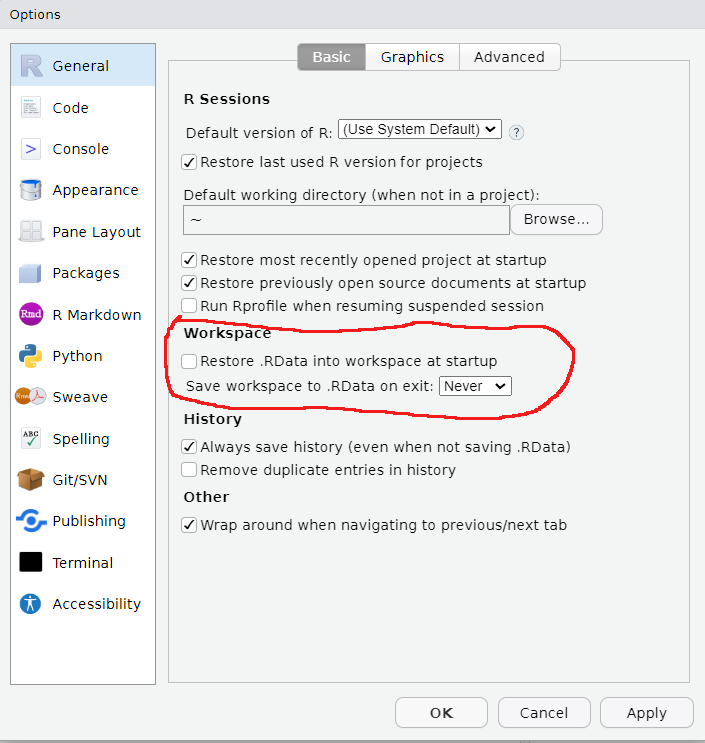
\includegraphics[width=\textwidth]{globaloptions}
\colc
\end{frame}


\bfr{R projects}
\begin{itemize}
\item Remembers settings, history, {\em etc.}
\item Organizes all files, scripts, data, {\em etc.}
\item \fbox{\sf File}\arrow \fbox{\sf New Project}
\item Usually use a new directory
\item \fbox{\sf Create Project}
\end{itemize}
\end{frame}

\bfr{Working directory}
\begin{itemize}
\item Current working directory seen at top of console window
\item Default folder R looks in when loading scripts, data, etc.
\item Opening a project file automatically sets working directory
\item Can use \lst{getwd()} to identify working directory 
\item Can use \lst{setwd()} to change working directory
\end{itemize}
\end{frame}

\bfr{Directory structure}

\cola
\dirtree{%
.1 Root.
.2 data.
.3 raw\_data.
.3 processed\_data.
.3 metadata.
.2 R.
.2 Rmd.
.2 scripts.
.2 output.
}
\colb\small
\begin{itemize}
\item \verb|Root| holds the \verb|.Rproj| file
\item \verb|raw_data| holds data from the field that should not be edited
\item \verb|processed_data| holds data that has been cleaned up
\item \verb|metadata| holds text files describing how the data was collected, etc.
\item \verb|R| holds R functions of general utility
\item \verb|Rmd| holds Rmarkdown files
\item \verb|scripts| holds current work
\item \verb|output| holds plots, data summaries, etc.
\end{itemize}
\colc

\end{frame}

\bfr{File names}
\cola
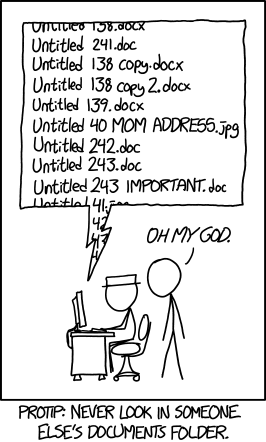
\includegraphics[width=0.667\textwidth]{xkcd_files}
\colb
\begin{itemize}
\item Short
\item Informative
\item No spaces
\item No special characters \verb|!@#$%^&*()|
\item Pad with zeros \verb|file001 file002 file003|
\item Use  ISO 8601 date format  \verb|YYYY-MM-DD or YYYYMMDD|
\end{itemize}
\colc

\end{frame}

\bfr{R script meta information}
\begin{lstlisting}[basicstyle=\tiny]
# Title: Time series analysis of snouters

# Purpose : This script performs a time series analyses on 
#           snouter count data.
#           Data consists of counts of snouter species 
#           collected from 18 islands in the Hy-yi-yi 
#           archipelago between 1950 and 1957. 
#           For details of snouter biology see:
#           https://en.wikipedia.org/wiki/Rhinogradentia

# Project number: #007

# DataFile:'data/snouter_pop.txt'

# Author: A. Nother
# Contact details: a.nother@uir.ac.uk

# Date script created: Mon Dec 2 16:06:44 2019 -----------
# Date script last modified: Thu Dec 12 16:07:12 2019 ----

# package dependencies
library(PopSnouter)
library(ggplot2)

print('put your lovely R code here')

# good practice to include session information

xfun::session_info()
\end{lstlisting}
\end{frame}

\bfr{Style guide}

\url{https://google.github.io/styleguide/Rguide.html}

\end{frame}
\bfr{Citing R}
\begin{lstlisting}[basicstyle=\tiny]
> citation()

To cite R in publications use:

  R Core Team (2021). R: A language and environment for
  statistical computing. R Foundation for Statistical
  Computing, Vienna, Austria. URL https://www.R-project.org/.

A BibTeX entry for LaTeX users is

  @Manual{,
    title = {R: A Language and Environment for Statistical Computing},
    author = {{R Core Team}},
    organization = {R Foundation for Statistical Computing},
    address = {Vienna, Austria},
    year = {2021},
    url = {https://www.R-project.org/},
  }

We have invested a lot of time and effort in creating R,
please cite it when using it for data analysis. See also
`citation("pkgname")' for citing R packages.
\end{lstlisting}
\end{frame}

\bfr{Exercise 1}
\end{frame}


\end{document}
